\usepackage[utf8]{inputenc}
\usepackage[T1]{fontenc}
\usepackage{mathptmx}
\usepackage[scaled=.90]{helvet}
\usepackage{courier}
\usepackage{caption}
\captionsetup{labelformat=empty,labelsep=none}
\usepackage{verbatim}
\usepackage{hyperref}
\usepackage{listings}
% strikethrough (\sout)
\usepackage{ulem}
\lstset{language=Perl,basicstyle=\normalsize,tabsize=3,showstringspaces=false}

\title{Dancer und DBIx::Class}
\author[racke]{Stefan Hornburg (Racke)\\ \texttt{racke@linuxia.de}}
\date{16. Deutscher Perl-Workshop, Hannover, 27. März 2013}

\begin{document}
\maketitle{}

\begin{frame}
  \titlepage
\end{frame}

\tableofcontents

% \section{Übersicht}

% DBIx::Class ist mit Sicherheit einer der größten Schätze von "Modern Perl"
% und bietet schnelle und komfortable Datenbankabfragen.

% Ebenso erleichtert Dancer das Erstellen von Webanwendungen mit einer leicht
% verständlichen Programmierung.

% Wie können beide zusammen genutzt werden? Zunächst mit dem DBIC Plugin für
% Dancer. Mit diesem können mehrere DBIx::Class Schemas innerhalb der
% Dancer-Anwendung verwenden werden.

% Um auch die Dancer-Sessions in der Datenbank zu speichern, habe ich eine Engine für Dancer und DBIC geschrieben.

% Außerdem werde ich ein Projekt vorstellen, mit dem man einfach den Inhalt
% von Datenbanken mittels eines DBIx::Class Schemas editieren kann.

% \begin{frame}<handout:0>{Übersicht}
% \begin{itemize}
% \item Einführung
% \item DBIC Schemas mit Dancer Plugin
% \item DBIC session engine
% \item Tabelleneditor
% \end{itemize}
% \end{frame}

% Wir starten mit einer kurzen Einführung von DBIx::Class.

\section{Produkte}
% \begin{frame}{Datenbank}
% \begin{itemize}
% \item Datenbank
% \item Tabellen
% \item Datensätze
% \end{itemize}
% \end{frame}

% \begin{frame}{DBIx::Class}
% \begin{itemize}
% \item Schema
% \item ResultSet
% \item Row / Objekt
% \end{itemize}
% \end{frame}

\subsection{Interchange6}
\begin{frame}{eCommerce Software}
\begin{itemize}
\item \sout{Magento}
\item Interchange6
\end{itemize}
\end{frame}

\subsection{TableEditor}
\begin{frame}{Datenbankadministration}
\begin{itemize}
\item \sout{phpmyadmin}
\item \sout{phppgadmin}
\item TableEditor
\end{itemize}
\end{frame}

\begin{frame}{TableEditor Features}
\begin{itemize}
\item Unterstützung mehrerer Datenbanksysteme
      MySQL, PostgreSQL
\item höherer Abstraktionslevel
\item modernes Frontend
\item wenig Quellcode
\end{itemize}
\end{frame}

Der TableEditor hat ein modernes Frontend. Es basiert
auf den Javascript-Paketen Bootstrap und Angular.
Die Templates und ein Teil der Logik sind somit Teil
des Frontends.

\subsection{TableEditor Demo}
\begin{frame}{TableEditor}
\begin{figure}
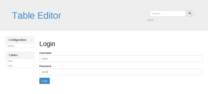
\includegraphics{images/te-login.png}
\caption{Anmeldung}
\end{figure}
\end{frame}

\section{Dancer::Plugin::DBIC}
\subsection{Anwendung}
\begin{frame}[fragile]{DBIx::Class ohne Dancer Plugin}
\begin{lstlisting}
use Interchange6::Schema;

$schema = Interchange6::Schema->connect(...);

$schema->resultset('User')->search({..});
\end{lstlisting}
\end{frame}

\begin{frame}[fragile]{DBIx::Class mit Dancer Plugin}
\begin{lstlisting}
use Dancer::Plugin::DBIC;

schema->resultset('User')->search({..});

resultset('User')->search({..});

rset('User')->search({..});
\end{lstlisting}
\end{frame}

\subsection{Konfiguration}

Im Normalfall verwendet man nur ein Schema in seiner
Dancer-Anwendung:

\begin{frame}[fragile]{Konfiguration}
\begin{lstlisting}
plugins:
  DBIC:
    default:
      dsn: dbi:mysql:interchange6
      user: racke
      pass: nevairbe
      schema_class: Interchange6::Schema
\end{lstlisting}
\end{frame}

Es sind aber auch mehrere möglich:

\begin{frame}[fragile]{Mehrere Schemas}
\begin{lstlisting}
plugins:
  DBIC:
    default:
      dsn: dbi:mysql:interchange6
      user: racke
      pass: nevairbe
      schema_class: Interchange6::Schema
    legacy:
      dsn: dbi:mysql:interchange5
      user: racke
      pass: nevairbe
      schema_class: Interchange5::Schema
\end{lstlisting}
\end{frame}

Das Schema \verb|legacy| wird dann wie folgt verwendet:

\begin{frame}[fragile]{Mehrere Schemas}
\begin{lstlisting}
use Dancer::Plugin::DBIC;

schema('legacy')->resultset('UserDb')->search({..});
\end{lstlisting}
\end{frame}

\subsection{UTF-8}
Im Gegensatz zu Dancer::Plugin::Database bietet das DBIC-Plugin
keine automatische Unterstützung für UTF-8. Also ist die entsprechende
DBI-Option in der Konfiguration einzutragen, hier für MySQL:
\begin{frame}[fragile]{UTF-8 für MySQL}
\begin{lstlisting}
plugins:
  DBIC:
    default:
      dsn: dbi:mysql:interchange6
      user: racke
      pass: nevairbe
      schema_class: Interchange6::Schema
      options:
        mysql_enable_utf8: 1
\end{lstlisting}
\end{frame}

Die Optionen für die gängigen Datenbanken in der Übersicht:

\begin{description}
\item[SQLite] \verb|sqlite_unicode: 1|
\item[MySQL] \verb|mysql_enable_utf8: 1|
\item[PostgreSQL] \verb|pg_enable_utf8: 1| 
\end{description}

\subsection{Schema dynamisch erzeugen}
Das DBIC-Plugin erzeugt dynamisch ein DBIx::Class::Schema, wenn
die Schema-Klasse (\verb|schema_class|) nicht angegeben wird.
Dazu ist das Modul DBIx::Class::Schema::Loader erforderlich.

Dies ist nicht empfehlenswert für den Produktionseinsatz, jedoch
praktisch für den Tabelleneditor.

\begin{frame}[fragile]{Schema dynamisch erzeugen}
\begin{itemize}
\item \verb|schema_class| fehlt in Konfiguration
\item DBIx::Class::Schema::Loader
\item Test und Entwicklung
\item TableEditor
\end{itemize}
\end{frame}

\section{Dancer::Session::DBIC}

\begin{frame}<handout:0>{Übersicht Dancer::Session::DBIC}
\begin{itemize}
\item Engines
\item Konfiguration
\item Serialisierung
\item Sitzungsablauf
\end{itemize}
\end{frame}

Dancer verwendet ``Engines'' für verschiedene Zwecke.
Dadurch kamen diese austauschen und das macht Dancer
weitaus flexibler. Die ``Engines'' werden entweder 
in der Konfiguration oder im Sourcecode mit dem \verb|set|
Schlüsselwort eingerichtet.

\subsection{Engines}
\begin{frame}{Engines}
\begin{itemize}
\item Templates \\
TT, Xslate, Flute, ...
\item Sitzungen (Sessions) \\ 
Storable, Database, DBIC
\item Logger \\
File, Syslog
\item Serialisierer  \\
JSON, YAML, XML
\end{itemize}
\end{frame}

Die Sessionengines werden in Dancer für gewöhnlich transparent
für den Anwendungscode in der Konfiguration eingerichtet:

\begin{frame}{Konfiguration}
\begin{description}
\item[session] Name der Sessionengine, hier DBIC
\item[session\_options] Optionen
\item[session\_expires] Ablaufzeit der Session
\end{description}
\end{frame}

Das ermöglicht es, auf dem Liveserver eine effizientere Engine
zu verwenden (z.B. Storable) und auf dem Entwicklungsserver
eine Engine, die einem beim debuggen hilft (z.B. YAML).

Die Optionen für Dancer::Session::DBIC ähneln der Konfiguration von
Dancer::Plugin::DBIC, zusätzlich können wir festlegen wie
die Sessions aus der Datenbank abgerufen werden können:

\begin{description}
\item[resultset] DBIx::Class resultset
\item[id\_column] primärer Schlüssel
\item[data\_column] Feld für Sitzungsdaten 
\end{description}

Das sieht dann z.B. für \href{https://metacpan.org/pod/Interchange6::Schema}{Interchange6::Schema} (Version 0.015) so aus:

\begin{frame}[fragile]{Konfiguration}
\begin{lstlisting}
session: "DBIC"
session_options:
  dsn: dbi:mysql:interchange6
  user: racke
  pass: nevairbe
  schema_class: Interchange6::Schema
  resultset: Session
  id_column: sessions_id
  data_column: session_data
session_expires: 12 hours
\end{lstlisting}
\end{frame}

Die Konfiguration kann aber ebenso im Hauptmodul
stattfinden:

\begin{frame}[fragile]{Konfiguration}
\begin{lstlisting}
set session => 'DBIC';
set session_options => {schema => schema};
\end{lstlisting}
\end{frame}

\subsection{Beispieltabelle}

Folgendermaßen sieht die Tabelle \verb|sessions| aus,
die vom Schema \href{https://metacpan.org/pod/Interchange6::Schema}{Interchange6::Schema} (Version 0.015)
erzeugt wird:

\begin{frame}[fragile]{Beispieltabelle}
\begin{lstlisting}
CREATE TABLE `sessions` (
  `sessions_id` varchar(255) NOT NULL,
  `session_data` text NOT NULL,
  `created` datetime NOT NULL,
  `last_modified` datetime NOT NULL,
  PRIMARY KEY (`sessions_id`)
) ENGINE=InnoDB;
\end{lstlisting}
\end{frame}

\subsection{Serialisierer}
\begin{frame}[fragile]{Serialisierer}
\begin{lstlisting}
set 'session_options' => {
    schema       => schema,
    serializer   => sub { YAML::Dump(@_); },
    deserializer => sub { YAML::Load(@_); },
};
\end{lstlisting}
\end{frame}

\subsection{Sitzungsablauf}

Beim Überschreiten der erlaubten Ablaufzeit wird die Sitzung
ungültig, sie wird jedoch nicht in der Datenbank gelöscht.
Dafür ist ein Skript zur regelmäßigen Löschung der
abgelaufenen Datensätze erforderlich.

JSON
andere DBIC connection?
tests?

\section{TableEditor}

\begin{frame}<handout:0>{Übersicht TableEditor}
\begin{itemize}
\item Installation
\item Frontend
\item Anmeldung
\item Beziehungen
\item Einschränkungen
\item Konfiguration
\end{itemize}
\end{frame}

\subsection{Installation}
Im günstigsten Fall kann die Installation mit 4 Schritten
erledigt werden:

\begin{frame}[fragile]{Installation}
\begin{lstlisting}
git clone https://github.com/interchange/TableEditor
cd TableEditor
cpanm .
./bin/app.pl
\end{lstlisting}
\end{frame}

\begin{frame}[fragile]{Treiber}
\begin{itemize}
\item DBD::mysql
\item DBD::Pg
\item ...
\end{itemize}
\end{frame}

\subsection{Frontend}
Das Frontend für den TableEditor ist mit Angular und Bootstrap erstellt.
Das Theme kann sehr einfach durch Austausch der CSS-Datei für Bootstrap
geändert werden.

\begin{frame}<handout:0>{Frontend}
\begin{itemize}
\item Angular
\item Bootstrap
\item Theme
\end{itemize}
\end{frame}

\subsection{Anmeldung}

Für die Integration von Authentifizierung in eine Dancer-Anwendung empfehlen
wir wärmestens das
\href{https://metacpan.org/pod/Dancer::Plugin::Auth::Extensible}{Auth::Extensible}
Plugin.

\begin{frame}{Anmeldung}
\begin{itemize}
\item Dancer::Plugin::Auth::Extensible
\item Provider
\begin{itemize}
\item Unix
\item DBIC
\end{itemize}
\item Datenbank \textit{(geplant)}
\end{itemize}
\end{frame}

\subsection{Beziehungen}

Beziehungen werden automatisch angezeigt.

\begin{frame}{Beziehungen}
\begin{itemize}
\item might\_have
\item has\_many
\item belongs\_to
\item many\_to\_many
\end{itemize}
\end{frame}

Filter

Es fehlen Felder in related orderline (Übersicht)

Different DBIC keys

Paging

\subsection{Einschränkungen}
\begin{frame}{Einschränkungen}
\begin{itemize}
\item Primärschlüssel für \textbf{eine} Spalte
\item Geschwindigkeit (komplexe Schemas)
\item Fehlerbehandlung
\end{itemize}
\end{frame}

\subsection{Konfiguration}
\begin{frame}
\begin{itemize}
\item Auth::Extensible
\item DBIC
% \begin{itemize}
% \item \verb|default|
% \end{itemize}
\end{itemize}
\end{frame}

\begin{frame}{Weitere Features}
\begin{itemize}
\item Suche (Solr)
\item Auswahl Schema
\end{itemize}
\end{frame}

\section{Ausblick und Mitarbeit}

\subsection{Entwicklung}

Das Git-Repository für den TableEditor befindet sich auf Github:

\begin{frame}{Entwicklung}
\url{https://github.com/interchange/TableEditor}
\end{frame}

\subsection{Dancer2}

Was ist mit Dancer2 ?

Für Dancer2 existiert bereits ein Plugin:

\url{https://metacpan.org/pod/Dancer2::Plugin::DBIC}

Die Sessionengine und der TableEditor wurden noch nicht auf Dancer2 portiert.

\begin{frame}{Dancer2}
  \begin{description}
  \item[Plugin::DBIC] \url{https://metacpan.org/pod/Dancer2::Plugin::DBIC}
  \item[Session::DBIC] noch nicht portiert
  \item[TableEditor] noch nicht portiert
  \end{description}
\end{frame}

% \section{Testing}
% DBIC, Plugin
% Testdatabase

\subsection{Slides}

\begin{frame}{Slides}
Slides:
\url{http://www.linuxia.de/talks/pws2014/dancer-dbic-de-beamer.pdf}
\end{frame}

\end{document}

%%% Local Variables: 
%%% mode: latex
%%% TeX-master: t
%%% End: 
